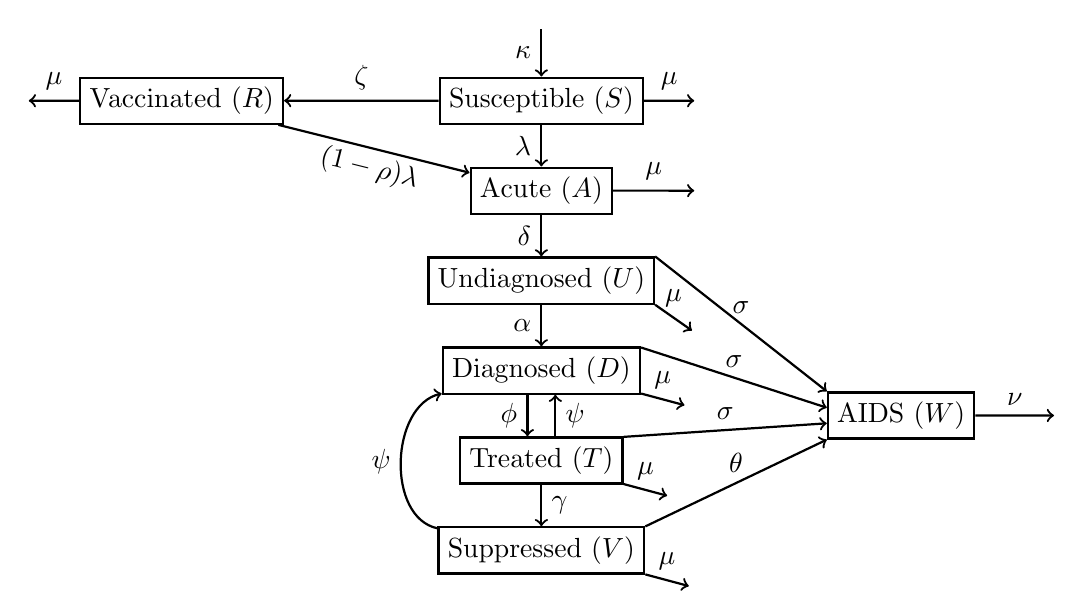
\begin{tikzpicture}[
  thick,
  scale = 1.142,
  compartment/.style = {draw},
  ]

  \node at (0, 5)
  [compartment, name = Susceptible] {Susceptible ($S$)};

  \node at (-4, 5)
  [compartment, name = Vaccinated] {Vaccinated ($R$)};

  \node at (0, 4)
  [compartment, name = Acute] {Acute ($A$)};

  \node at (0, 3)
  [compartment, name = Undiagnosed] {Undiagnosed ($U$)};

  \node at (0, 2)
  [compartment, name = Diagnosed] {Diagnosed ($D$)};

  \node at (0, 1)
  [compartment, name = Treated] {Treated ($T$)};

  \node at (0, 0)
  [compartment, name = Suppressed] {Suppressed ($V$)};

  \node at (4, 1.5)
  [compartment, name = AIDS] {AIDS ($W$)};

  \draw [->] (Susceptible) to node [left] {$\lambda$} (Acute);

  \draw [->] (Susceptible) to node [above] {$\zeta$} (Vaccinated);

  \draw [->] (Vaccinated) to node [sloped, below, yshift = 0.05cm] {$(1 - \rho) \lambda$} (Acute);

  \draw [->] (Acute) to node [left] {$\delta$} (Undiagnosed);

  \draw [->] (Undiagnosed) to node [left] {$\alpha$} (Diagnosed);

  \draw [->] (Diagnosed.240) to node [left] {$\phi$} (Treated.120);

  \draw [->] (Treated.60) to node [right] {$\psi$} (Diagnosed.300);

  \draw [->] (Treated) to node [right] {$\gamma$} (Suppressed);

  \draw [->] (Suppressed) to [out = 168, in = 193] node [left] {$\psi$} (Diagnosed);

  \draw [->] (Undiagnosed.12) to node [above] {$\sigma$} (AIDS.162);

  \draw [->] (Diagnosed.13) to node [above] {$\sigma$} (AIDS.174);

  \draw [->] (Treated.16) to node [above] {$\sigma$} (AIDS.186);

  \draw [->] (Suppressed.13) to node [above] {$\theta$} (AIDS.198);

  \draw [<-] (Susceptible) to node [left] {$\kappa$} +(90: 0.8);

  \draw [->] (Susceptible) to node [above] {$\mu$} +(0: 1.7);

  \draw [->] (Vaccinated) to node [above] {$\mu$} +(0: -1.7);

  \draw [->] (Acute) to node [above] {$\mu$} +(0: 1.7);

  \draw [->] (Undiagnosed.348) to node [above] {$\mu$} +(325: 0.5);

  \draw [->] (Diagnosed.347) to node [above] {$\mu$} +(345: 0.5);

  \draw [->] (Treated.344) to node [above] {$\mu$} +(345: 0.5);

  \draw [->] (Suppressed.347) to node [above] {$\mu$} +(345: 0.5);

  \draw [->] (AIDS) to node [above] {$\nu$} +(0: 1.7);

\end{tikzpicture}


%%% Local Variables:
%%% mode: latex
%%% TeX-master: "supporting_information"
%%% End:
